\changecolours{ScoutNavy}
\section{Variações Avançadas dos Comandos SET e GET}

% ------------------------------------------------------------------------------
\twocolframe[title={Problema Real Inicial: Cache de Termos de Busca},leftcol=7cm,rightcol=7cm]{%
  \alert{O Gargalo de Consultas Textuais}\par
  \itemseps[topsepi=2mm,itemsepi=3mm,labelsep=2mm,leftmargini=4mm]
  \begin{itemize}
    \item No e-commerce da Tauá Tech Store, milhares de clientes pesquisam simultaneamente por \textit{``notebook dell''}.
    \item Realizar buscas em bancos relacionais com \texttt{LIKE '\%notebook\%'} ou regex no MongoDB exige varredura pesada e leva de 150 a 250 ms.
    \item \textbf{Modelagem Chave-Valor:}
    \item \textbf{Chave:} \texttt{busca:termo:notebook\_dell}
    \item \textbf{Valor:} JSON com lista de produtos encontrados.
  \end{itemize}
}{%
  \alert{A Estratégia de Aceleração}\par
  \itemseps[topsepi=2mm,itemsepi=3mm,labelsep=2mm,leftmargini=4mm]
  \begin{itemize}
    \item Armazena o resultado em memória no Redis com TTL de 300 segundos (\textbf{5 minutos}).
    \item \textbf{Cache Hit:} A resposta é devolvida em \textbf{0,07 ms} ($\approx 2800\times$ mais rápido!).
    \item \textbf{Cache Miss:} Primeira consulta calcula no banco e alimenta o Redis.
    \item Contadores atômicos com \texttt{INCR} medem a popularidade de cada termo em tempo real.
  \end{itemize}
}

% ------------------------------------------------------------------------------
\begin{frame}{Ciclo de Vida do Cache de Busca no E-commerce}
  \centering
  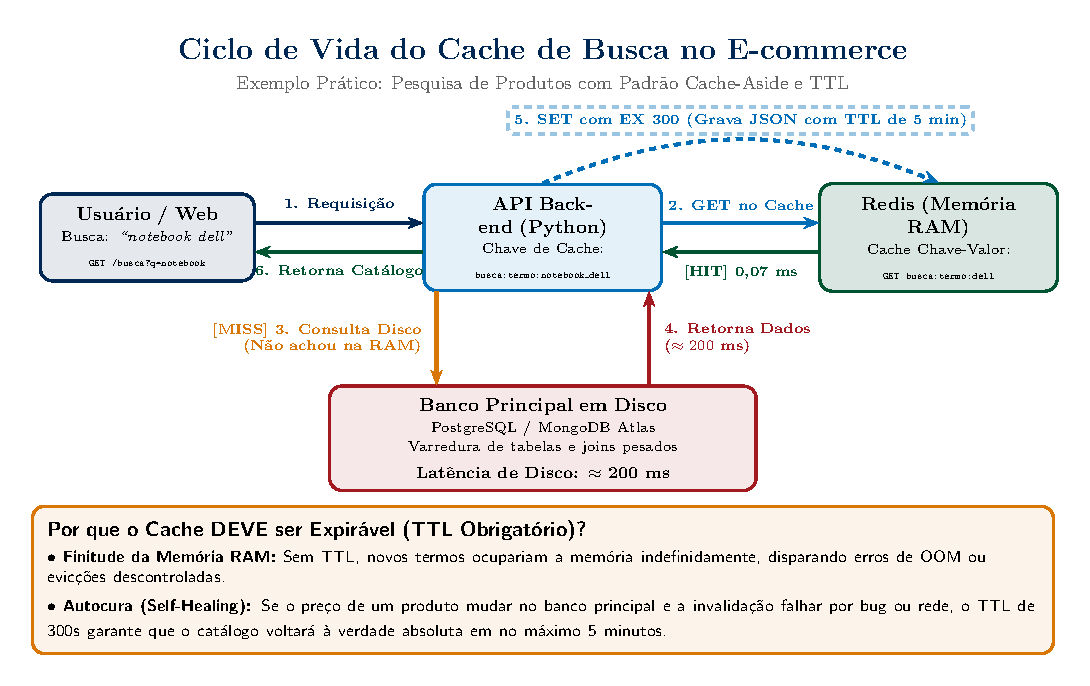
\includegraphics[width=0.90\textwidth,height=0.74\textheight,keepaspectratio]{figuras/fig_ciclo_cache_busca.pdf}
\end{frame}

% ------------------------------------------------------------------------------
\begin{frame}[fragile]{SET com Expiração Temporal (EX e PX)}
  \begin{columns}[T]
    \begin{column}{0.48\textwidth}
      \alert{Expiração Temporal (TTL)}\par
      \itemseps[topsepi=1mm,itemsepi=1.5mm,labelsep=2mm,leftmargini=4mm]
      \small
      \begin{itemize}
        \item O parâmetro \texttt{EX} define a expiração em segundos inteiros.
        \item O parâmetro \texttt{PX} define a expiração em milissegundos.
        \item Evita acúmulo descontrolado de dados obsoletos na memória RAM.
      \end{itemize}
    \end{column}
    \begin{column}{0.50\textwidth}
      \alert{Comandos no redis-cli}\par
      \begin{lstlisting}[language=bash]
# Gravar catalogo com TTL de 300s (5 min):
127.0.0.1:6379> SET busca:dell "[{id:1}]" EX 300
OK

# Consultar TTL restante em segundos:
127.0.0.1:6379> TTL busca:dell
(integer) 298

# Gravar chave com PX (2500 ms):
127.0.0.1:6379> SET ping:host "10.0.0.1" PX 2500
OK
      \end{lstlisting}
    \end{column}
  \end{columns}
\end{frame}

% ------------------------------------------------------------------------------
\begin{frame}[fragile]{SET com Trava Distribuída (Lock NX)}
  \begin{columns}[T]
    \begin{column}{0.48\textwidth}
      \alert{Exclusão Mútua Atômica}\par
      \itemseps[topsepi=1mm,itemsepi=1.5mm,labelsep=2mm,leftmargini=4mm]
      \small
      \begin{itemize}
        \item O modificador \texttt{NX} grava \textbf{apenas se a chave não existir}.
        \item Se a chave já existir, a gravação falha e devolve \texttt{(nil)}.
        \item \textbf{Caso Real:} Trava de concorrência para reservar a última unidade de um estoque.
      \end{itemize}
    \end{column}
    \begin{column}{0.50\textwidth}
      \alert{Comandos no redis-cli}\par
      \begin{lstlisting}[language=bash]
# Worker A adquire a trava por 15s:
127.0.0.1:6379> SET lock:prod:101 "wA" NX EX 15
OK

# Worker B tenta simultaneamente:
127.0.0.1:6379> SET lock:prod:101 "wB" NX EX 15
(nil)  # Bloqueado com sucesso!

# Liberacao manual da trava:
127.0.0.1:6379> DEL lock:prod:101
(integer) 1
      \end{lstlisting}
    \end{column}
  \end{columns}
\end{frame}

% ------------------------------------------------------------------------------
\begin{frame}[fragile]{SET Condicional (XX) e Preservação de TTL (KEEPTTL)}
  \begin{columns}[T]
    \begin{column}{0.48\textwidth}
      \alert{Atualização Estrita e TTL}\par
      \itemseps[topsepi=1mm,itemsepi=1.5mm,labelsep=2mm,leftmargini=4mm]
      \small
      \begin{itemize}
        \item \texttt{XX}: Grava \textbf{apenas se a chave já existir} (útil para atualizar status sem criar lixo).
        \item \texttt{KEEPTTL}: Atualiza o conteúdo da chave preservando a contagem de tempo restante.
      \end{itemize}
    \end{column}
    \begin{column}{0.50\textwidth}
      \alert{Comandos no redis-cli}\par
      \begin{lstlisting}[language=bash]
# Tentar atualizar chave inexistente:
127.0.0.1:6379> SET status:servico "on" XX
(nil)  # Nao cria chave nova

# Criar sessao com TTL de 60s:
127.0.0.1:6379> SET sessao:u1 "token_v1" EX 60
OK

# Atualizar valor mantendo o tempo:
127.0.0.1:6379> SET sessao:u1 "token_v2" KEEPTTL
OK  # O relogio regressivo nao zera!
      \end{lstlisting}
    \end{column}
  \end{columns}
\end{frame}

% ------------------------------------------------------------------------------
\begin{frame}[fragile]{SET com Troca Atômica (GET) e Lotes (MSET)}
  \begin{columns}[T]
    \begin{column}{0.48\textwidth}
      \alert{Substituição e Multi-Escrita}\par
      \itemseps[topsepi=1mm,itemsepi=1.5mm,labelsep=2mm,leftmargini=4mm]
      \small
      \begin{itemize}
        \item \texttt{SET ... GET}: Atualiza o valor e devolve o valor anterior atomicamente.
        \item \texttt{MSET}: Grava múltiplas chaves e valores em um único pacote TCP.
        \item Evita múltiplas viagens de ida e volta (RTT).
      \end{itemize}
    \end{column}
    \begin{column}{0.50\textwidth}
      \alert{Comandos no redis-cli}\par
      \begin{lstlisting}[language=bash]
# Substituir valor e receber o antigo:
127.0.0.1:6379> SET contagem:vendas 100 GET
"85"  # Retornou o valor anterior!

# Gravar varias moedas em 1 RTT:
127.0.0.1:6379> MSET usd 5.45 eur 5.95 btc 345k
OK

# Leitura conjunta imediata:
127.0.0.1:6379> MGET usd eur
1) "5.45"  2) "5.95"
      \end{lstlisting}
    \end{column}
  \end{columns}
\end{frame}

% ------------------------------------------------------------------------------
\begin{frame}[fragile]{GET Simples e em Lote (MGET)}
  \begin{columns}[T]
    \begin{column}{0.48\textwidth}
      \alert{Recuperação de Alta Velocidade}\par
      \itemseps[topsepi=1mm,itemsepi=1.5mm,labelsep=2mm,leftmargini=4mm]
      \small
      \begin{itemize}
        \item \texttt{GET}: Recupera uma única chave em $\mathcal{O}(1)$.
        \item \texttt{MGET}: Recupera múltiplas chaves de forma atômica.
        \item Chaves inexistentes retornam \texttt{(nil)} sem interromper a consulta das demais.
      \end{itemize}
    \end{column}
    \begin{column}{0.50\textwidth}
      \alert{Comandos no redis-cli}\par
      \begin{lstlisting}[language=bash]
# Leitura simples de termo cacheado:
127.0.0.1:6379> GET busca:dell
"[{id:1}]"

# Consulta de multiplas chaves:
127.0.0.1:6379> MGET usd eur chave_inexistente
1) "5.45"
2) "5.95"
3) (nil)
      \end{lstlisting}
    \end{column}
  \end{columns}
\end{frame}

% ------------------------------------------------------------------------------
\begin{frame}[fragile]{GETDEL: Consumo Atômico de Tokens de Uso Único}
  \begin{columns}[T]
    \begin{column}{0.48\textwidth}
      \alert{Leitura e Destruição em $\mathcal{O}(1)$}\par
      \itemseps[topsepi=1mm,itemsepi=1.5mm,labelsep=2mm,leftmargini=4mm]
      \small
      \begin{itemize}
        \item Lê o valor e \textbf{remove a chave atomicamente} em uma única operação.
        \item Elimina vulnerabilidade de reutilização concorrente (*double spending*).
        \item \textbf{Casos Reais:} Cobrança PIX, tokens de redefinição de senha e ingressos.
      \end{itemize}
    \end{column}
    \begin{column}{0.50\textwidth}
      \alert{Comandos no redis-cli}\par
      \begin{lstlisting}[language=bash]
# Gerar token PIX de 60 segundos:
127.0.0.1:6379> SET token:pix:99 "R$500" EX 60
OK

# Consumir e apagar atomicamente:
127.0.0.1:6379> GETDEL token:pix:99
"R$500"

# Segunda tentativa de leitura:
127.0.0.1:6379> GET token:pix:99
(nil)  # Ja consumido e destruido!
      \end{lstlisting}
    \end{column}
  \end{columns}
\end{frame}

% ------------------------------------------------------------------------------
\begin{frame}[fragile]{GETEX: Renovação Deslizante de Sessão}
  \begin{columns}[T]
    \begin{column}{0.48\textwidth}
      \alert{Extensão de Vida na Leitura}\par
      \itemseps[topsepi=1mm,itemsepi=1.5mm,labelsep=2mm,leftmargini=4mm]
      \small
      \begin{itemize}
        \item \texttt{GETEX}: Lê o dado e atualiza o seu TTL no mesmo instante.
        \item \textbf{Sessão Deslizante:} Enquanto o usuário navega na aplicação, a expiração é postergada sem comandos adicionais de escrita.
      \end{itemize}
    \end{column}
    \begin{column}{0.50\textwidth}
      \alert{Comandos no redis-cli}\par
      \begin{lstlisting}[language=bash]
# Sessao com TTL de 30s:
127.0.0.1:6379> SET sessao:u42 "jwt_token" EX 30
OK

# Ler e estender para 1800s (30m):
127.0.0.1:6379> GETEX sessao:u42 EX 1800
"jwt_token"

# Verificar novo tempo de expiracao:
127.0.0.1:6379> TTL sessao:u42
(integer) 1799
      \end{lstlisting}
    \end{column}
  \end{columns}
\end{frame}

% ------------------------------------------------------------------------------
\begin{frame}[fragile]{Inspeção de Strings (GETRANGE e STRLEN)}
  \begin{columns}[T]
    \begin{column}{0.48\textwidth}
      \alert{Substrings e Tamanho em Bytes}\par
      \itemseps[topsepi=1mm,itemsepi=1.5mm,labelsep=2mm,leftmargini=4mm]
      \small
      \begin{itemize}
        \item \texttt{GETRANGE}: Extrai intervalo de caracteres usando offsets de início e fim.
        \item \texttt{STRLEN}: Retorna o tamanho exato da string armazenada em bytes.
        \item Execução instantânea em memória.
      \end{itemize}
    \end{column}
    \begin{column}{0.50\textwidth}
      \alert{Comandos no redis-cli}\par
      \begin{lstlisting}[language=bash]
# Gravar mensagem textual:
127.0.0.1:6379> SET msg "IFCE Campus Taua"
OK

# Obter substring pelo intervalo [5, 10]:
127.0.0.1:6379> GETRANGE msg 5 10
"Campus"

# Medir comprimento em bytes:
127.0.0.1:6379> STRLEN msg
(integer) 16
      \end{lstlisting}
    \end{column}
  \end{columns}
\end{frame}
